\begin{tikzpicture}[
    x=1cm, y=1cm,
    every node/.style={font=\normalsize}
]
    % Stavy
    \initialstate{q0}{(0,0)}{$q_0$}{(-1.1,0)}{west}
    \state{q1}{(1.8,0)}{$q_1$}
    \state{q2}{(3.6,0)}{$q_2$}
    \acceptingstate{q3}{(5.4,0)}{$q_3$}

    % Přechody
    \transitionarrow[loop below]{q0}{below}{$0,1$}{q0}
    \transitionarrow{q0}{above}{$1$}{q1}
    \transitionarrow{q1}{above}{$0$}{q2}
    \transitionarrow{q2}{above}{$1$}{q3}
    \transitionarrow[loop above]{q3}{above}{$0,1$}{q3}
\end{tikzpicture}